\section{Data}

 \frame{\sectionpage}

\begin{frame}{Sample}
    \begin{itemize}
        \item {\color{frenchlilac!45!white}\underline{\textit{Candidates}}}: \underline{\textbf{113777}} profiles
        
        \item {\color{frenchlilac!45!white}\underline{\textit{Employers}}}: \underline{\textbf{463860}} interview requests for \textbf{\underline{39839}} jobs in \textbf{\underline{6532}} firms
        
        \item {\color{frenchlilac!45!white}\underline{\textit{Final offers}}}: \underline{\textbf{7582}} offers
        
        \vspace*{15pt}
        \item<2-> {\color{frenchlilac!45!white}\underline{\textit{Gender}}}: \underline{\textbf{20.8\%}} female
        \begin{itemize}
            \item[-] self declaration: 50\%
            \item[-] imputation of missing: 34.6\% (name prediction)
        \end{itemize}
        \item<3-> {\color{frenchlilac!45!white}\underline{\textit{Time window}}}
    \end{itemize}
\end{frame}

\begin{frame}{Candidates Summary}
    \begin{table}[h!]
        \footnotesize
        \begin{center}
            \label{tab:candidate_sum}
            \begin{tabular}{lccc}
                & All & Male & Female \\
               \hline
                Number of candidates & 113777 & \textcolor{frenchlilac!45!white}{76223} & 19998 \\
                Average number of bids received & 4.5 & \textcolor{frenchlilac!45!white}{4.6} & 4.2 \\
                Prob. of accepting an interview request & 62.2 & 62.0 & \textcolor{frenchlilac!45!white}{63.2}\\
                \hline
                \% bachelor & 97.6 & 97.3 & \textcolor{frenchlilac!45!white}{98.7} \\
                \% master & 41.4 & 40.3 & \textcolor{frenchlilac!45!white}{45.2} \\
                \% CS degree & 55.2 & \textcolor{frenchlilac!45!white}{57.2} & 47.7 \\
                \% IvyPlus degree & 9.4 & 8.7 & \textcolor{frenchlilac!45!white}{11.8} \\
                \hline 
                Years of experience & 11.3 & \textcolor{frenchlilac!45!white}{11.7} & 10.1 \\
                \% leading a team & 32.7 & \textcolor{frenchlilac!45!white}{33.8} & 27.6 \\
                \% employed & 73.1 & \textcolor{frenchlilac!45!white}{74.0} & 69.7 \\
                Days unemployed & 236.2 & 231.1 & \textcolor{frenchlilac!45!white}{253.2} \\
                \hline 
                \% software engineers & 61.7 & \textcolor{frenchlilac!45!white}{66.6} & 43.2 \\
                \% designers & 8.3 & 6.1 & \textcolor{frenchlilac!45!white}{16.6} \\
                \& product managers & 8.3& 7.5 & \textcolor{frenchlilac!45!white}{11.4}
            \end{tabular}
        \end{center}
    \end{table}
\end{frame}

\begin{frame}{Gender and Preferences over Firms}
    \begin{table}[h!]
        \footnotesize
        \begin{center}
            \label{tab:candidate_pref}
            \begin{tabular}{lcc}
                & Male & Female (relative) \\
               \hline
                No preferences & 0.252 & {+0.013} \\
                \hline
                \textcolor{frenchlilac!45!white}{\textit{Firm size}} & & \\
                16-50 & 0.432 & -0.031 \\
                201-500 & 0.433 & +0.009 \\
                500+ & 0.351 & +0.021 \\
                \hline 
                \textcolor{frenchlilac!45!white}{\textit{Industry}} & & \\
                Hardware IoT & 0.033 & -0.011 \\
                Finance & 0.041 & -0.007 \\
                Education & 0.026 & +0.005 \\
                Health-tech & 0.028 & +0.007 \\
                \hline
                \textcolor{frenchlilac!45!white}{\textit{Career Goal}} & &\\
                New technologies & 0.249 & -0.013 \\
                Mentorship & 0.090 & +0.006\\
                Socially Conscious & 0.088 & +0.023 
            \end{tabular}
        \end{center}
    \end{table}
\end{frame}

\begin{frame}{Company}
    
    \begin{table}[h!]
        \footnotesize
        \begin{center}
            \label{tab:firm}
            \begin{tabular}{lccc}
                & \multicolumn{3}{c}{Variables of Interest} \\
               \hline
                & No. jobs & No. bids per job & No. final offers \\
                & 39839 & 11.6 & 7582 \\
                \hline
                & Revenue & Firm age (yrs) & No. benefits \\
                mean & 708.4 & 9.04 & 8.49 \\
                median & 15 & 6 & 6 \\
                \hline 
                
            \end{tabular}
        \end{center}
    \end{table}

    \vspace*{10pt}
    Size distribution:
    \begin{table}[h!]
        \footnotesize
        \begin{center}
            \begin{tabular}{cccccc}
                1-10 & 11-50 & 51-200 & 201-500 & 501-1000 & 1000+ \\
                \hline 
               18\% & 29\% & 31\% & 11\% & 5\% & 6\%
            \end{tabular}
        \end{center}
    \end{table}
\end{frame}

\begin{frame}{Job and Candidate Search}
    \begin{itemize}
        \item<+-> candidate side:
        \begin{itemize}
            \item[-] length spell: \textcolor{frenchlilac!45!white}{\textbf{2}} (default) {\scriptsize \textit{(55\%)}} plus 2  {\scriptsize \textit{(22\%)}} to 4  {\scriptsize \textit{(23\%)}} weeks
            \item[-] number of spells: 1 {\scriptsize \textit{(84\%)}} / 2 {\scriptsize \textit{(11\%)}} / 3+ {\scriptsize \textit{(5\%)}}
            \item[-] attractiveness: \textcolor{frenchlilac!45!white}{\textbf{6.6}} interview requests for hired candicates (4.5 otherwise)
        \end{itemize}
        \item<+-> company side:
        \begin{itemize}
            \item[-] sample: jobs that find a match on the platform
            \item[-] number of hirings: 1 {\scriptsize \textit{(77.3\%)}} / 2 {\scriptsize \textit{(14.3\%)}} / 3+ {\scriptsize \textit{(8.4\%)}}
            \item[-] search effort: \textcolor{frenchlilac!45!white}{\textbf{30.2}} interview requests for successful search (\textcolor{frenchlilac!45!white}{\textbf{11.6}} otherwise) 
        \end{itemize}
    \end{itemize}
\end{frame}

\begin{frame}{Ask Salary: Could it be Strategic Revealing?}
    Key: Ask Salary is a \textcolor{frenchlilac!45!white}{\textit{\underline{signal} to firms}}
    \uncover<2->{
        \begin{center}
            \begin{tikzpicture}[every node/.append style={font=\small}]
                % Draw the axes
                \draw [white, very thick] (-6,0) -- (6,0) node[right]{wage};
                \draw [white, very thick] (0,0.2) -- (0,-0.2) node[below]{$\text{salary}_{\text{ask}}$};

                \uncover<3->{\draw [white, very thick] (4,-0.2) -- (4,0.2);
                \draw[decorate,decoration={brace,amplitude=5pt,raise=5pt},yshift=0pt, very thick, color=frenchlilac!45!white] (0,0) -- (4,0) node [midway, yshift=15pt, xshift =0pt]{\textit{reservation}};}
                
                \uncover<4->{\draw [white, very thick] (-4,-0.2) -- (-4,0.2);
                \draw[decorate,decoration={brace,amplitude=5pt,raise=5pt},yshift=0pt, very thick, color=frenchlilac!45!white] (-4,0) -- (0,0) node [midway, yshift=15pt, xshift =0pt]{\textit{bluffing}};}

                \uncover<5->{
                \draw [white, very thick] (2,-0.7) -- (2,0.2);
                \draw [white, very thick] (-2,-0.7) -- (-2,0.2);
                \draw[decorate,decoration={brace,amplitude=5pt,raise=20pt,mirror},yshift=0pt, very thick, color=frenchlilac!45!white] (-2,0) -- (2,0) node [midway, yshift=-29pt, xshift =0pt]{\textit{estimation}};
                }

                \uncover<6->{
                    \draw [->, frenchlilac!45!white, very thick] (-0.5,1) node[above]{$\boxed{\text{salary}_{\text{bid}}}$} -- (-0.5,0);
                }

            % Done
            \end{tikzpicture}
        \end{center}
    }
\end{frame}

\begin{frame}{Ask Salary: Could it be Strategic Revealing?}
    \begin{figure}
        \centering
        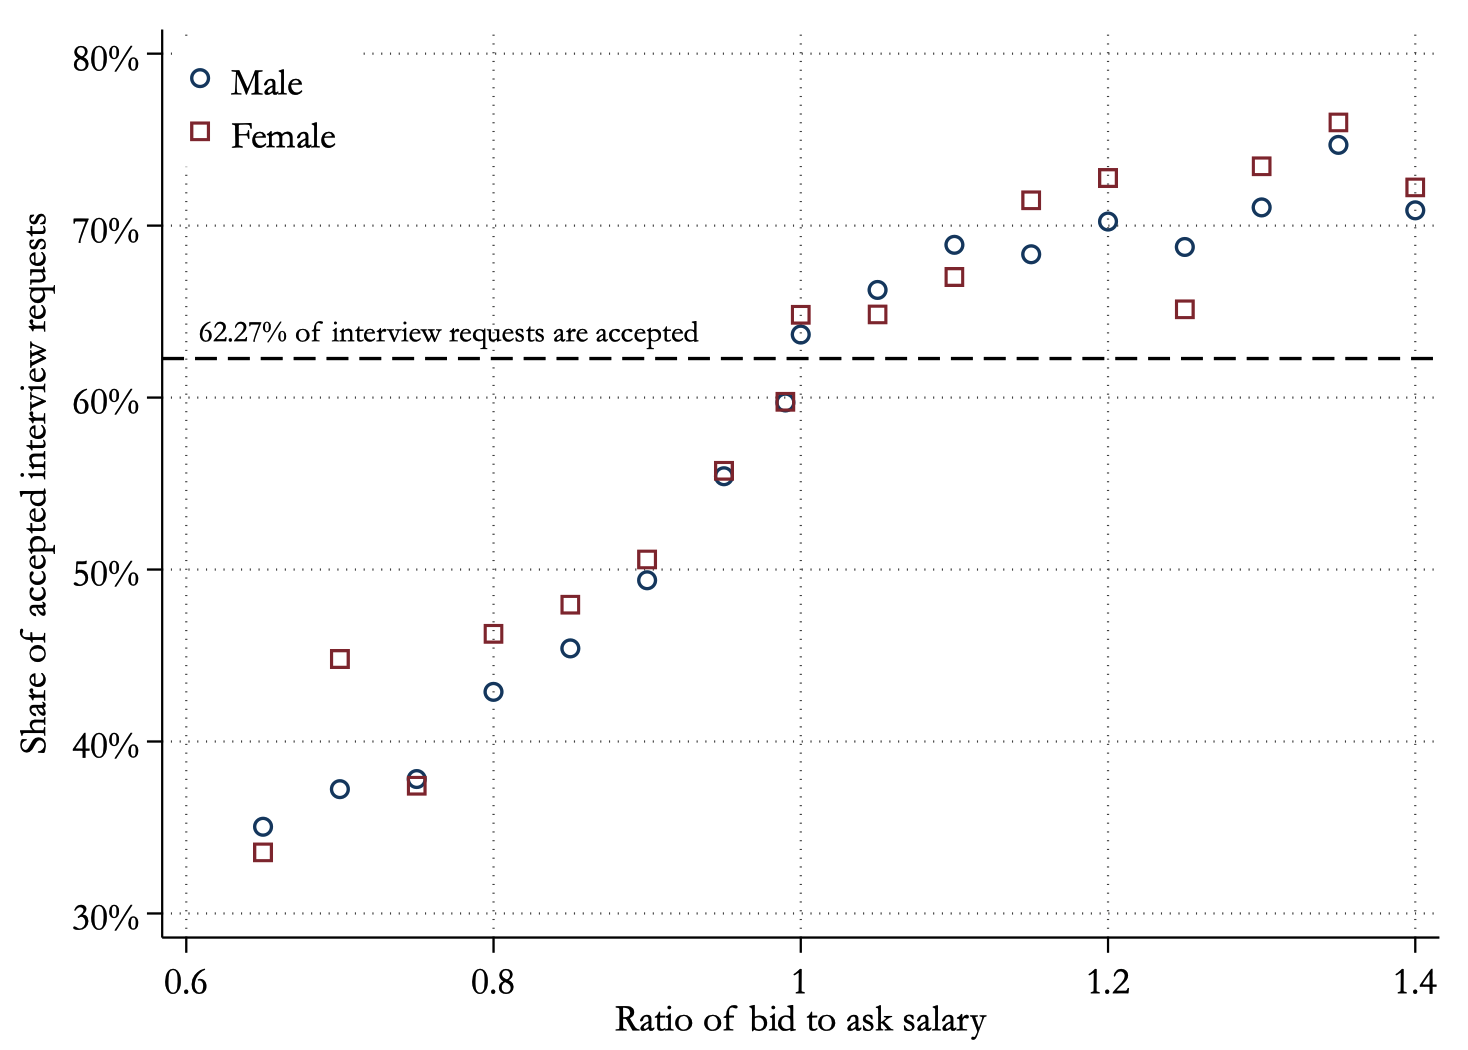
\includegraphics[height = 0.7 \textheight]{images/ask1.png}
    \end{figure}
\end{frame}

\begin{frame}{Expected Salary: Could it be Strategic Revealing?}
    \begin{figure}
        \centering
        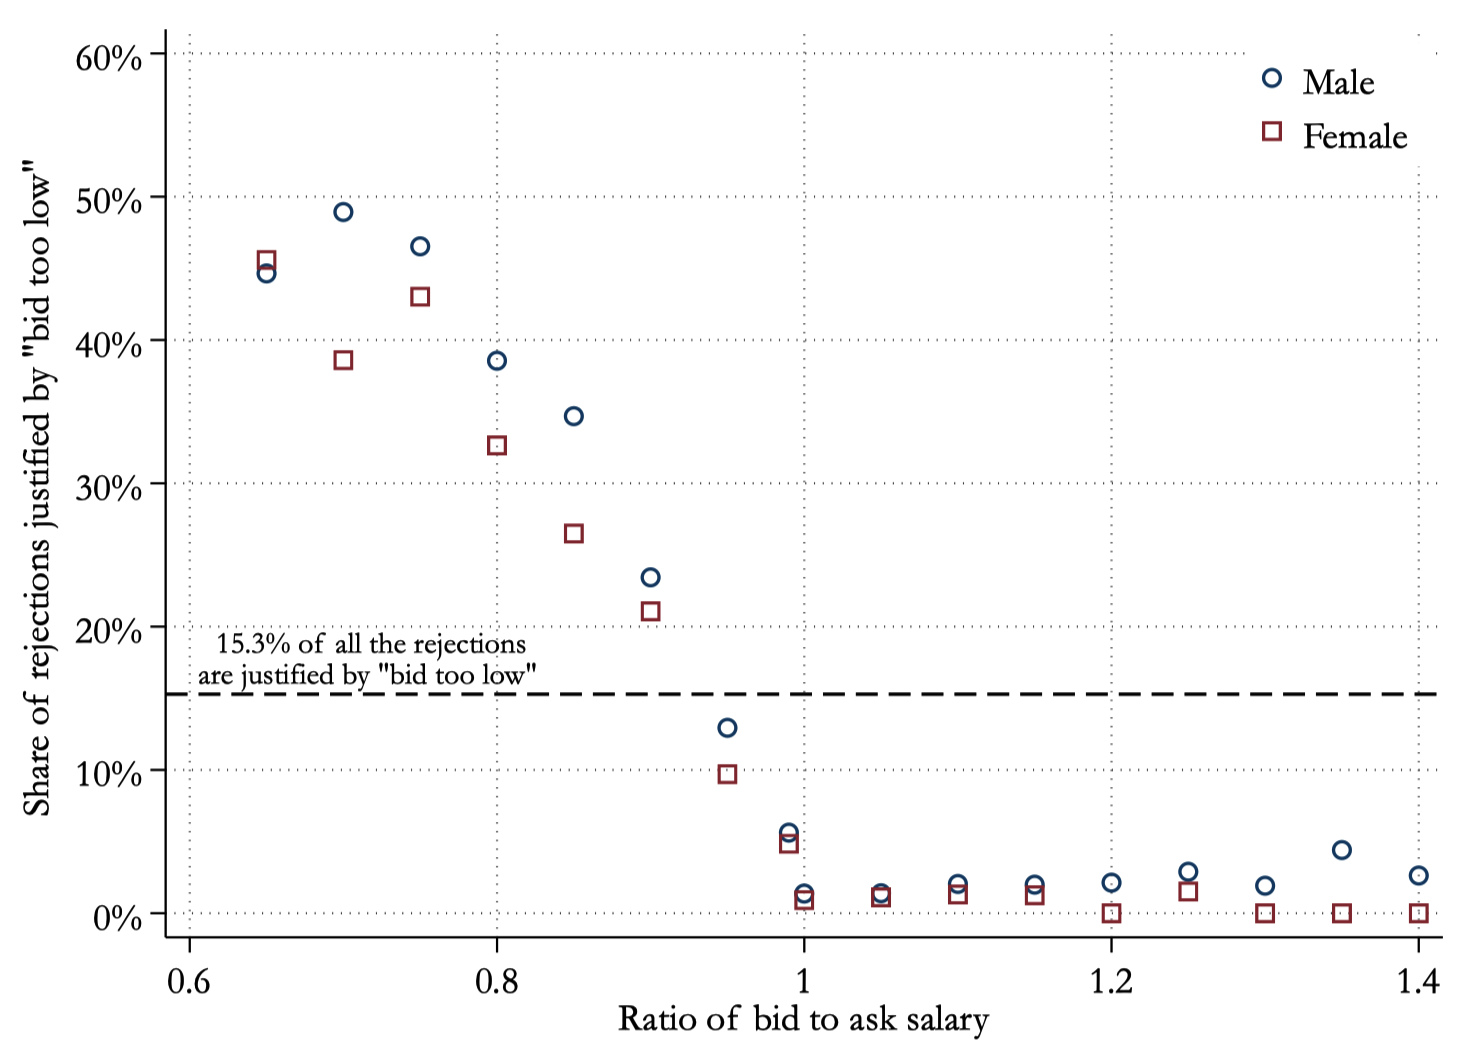
\includegraphics[height = 0.7 \textheight]{images/ask2.png}
    \end{figure}
\end{frame}

\begin{frame}{Bid Salary: Willingness to Pay or \textit{Decoy}?}
    \begin{columns}[T]
        \begin{column}{0.45\textwidth}
            \begin{figure}
                \centering
                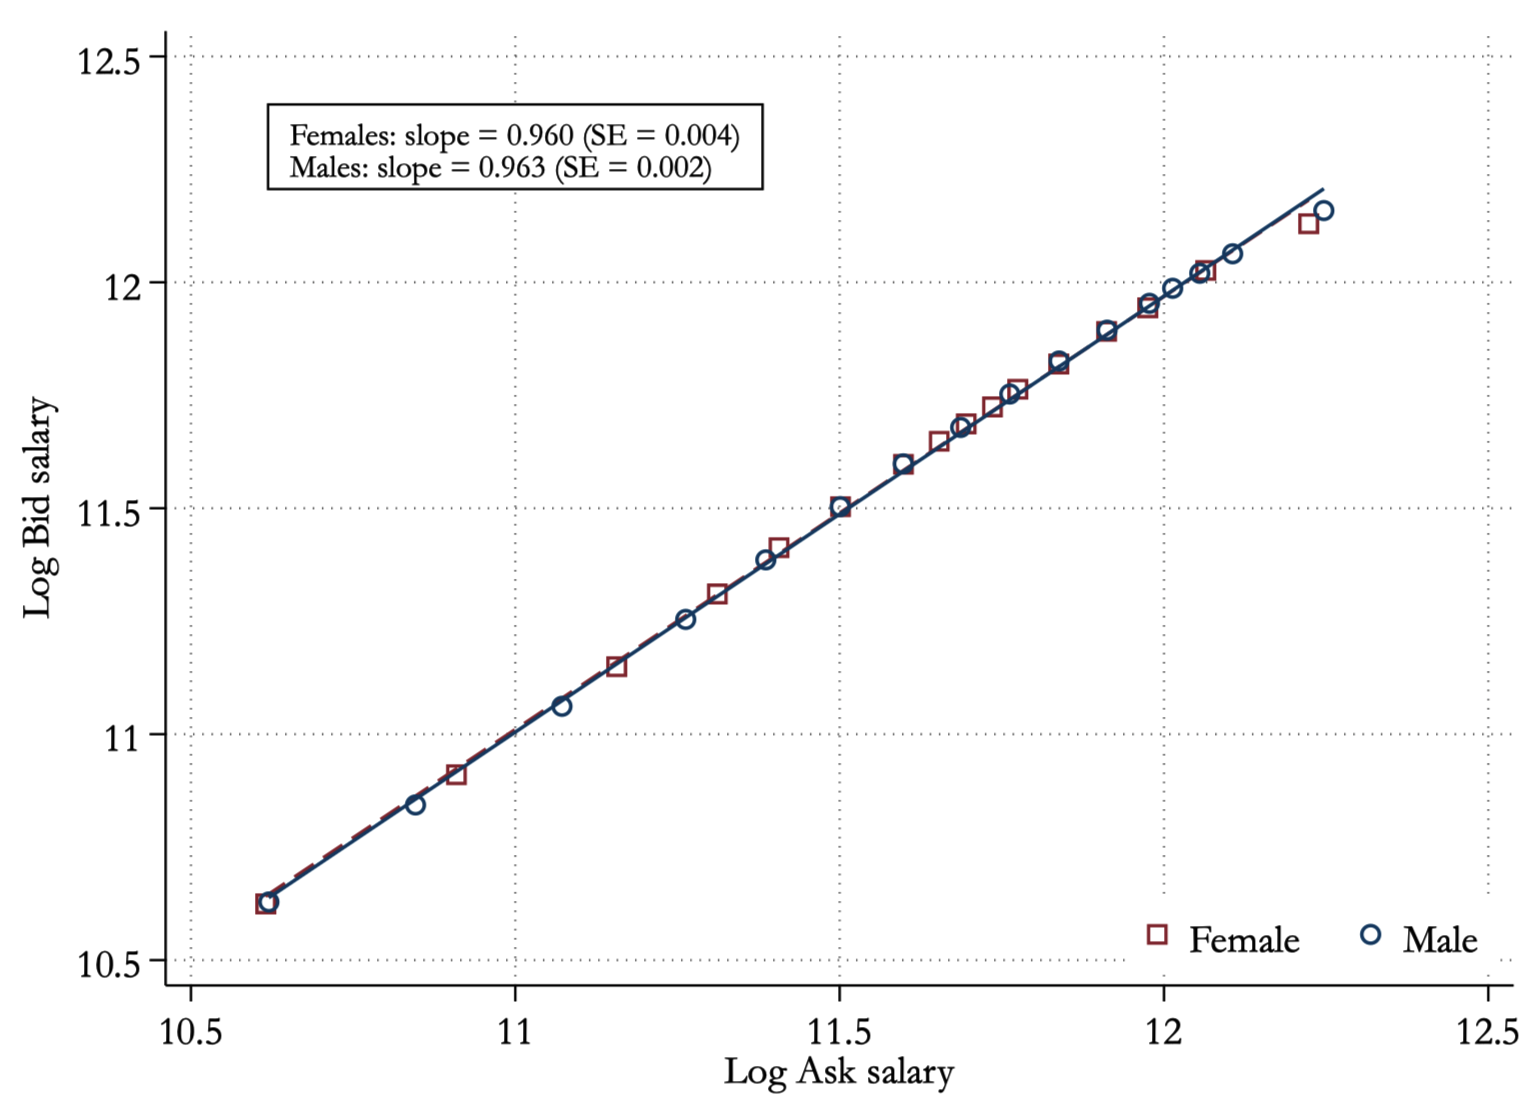
\includegraphics[width = 0.95 \textwidth]{images/ask3.png}
                {\footnotesize \textcolor{frenchlilac!45!white}{Ask} Salary - \textcolor{frenchlilac!45!white}{Bid} Salary}
            \end{figure}
        \end{column}

        \begin{column}{0.45\textwidth}
            \begin{figure}
                \centering
                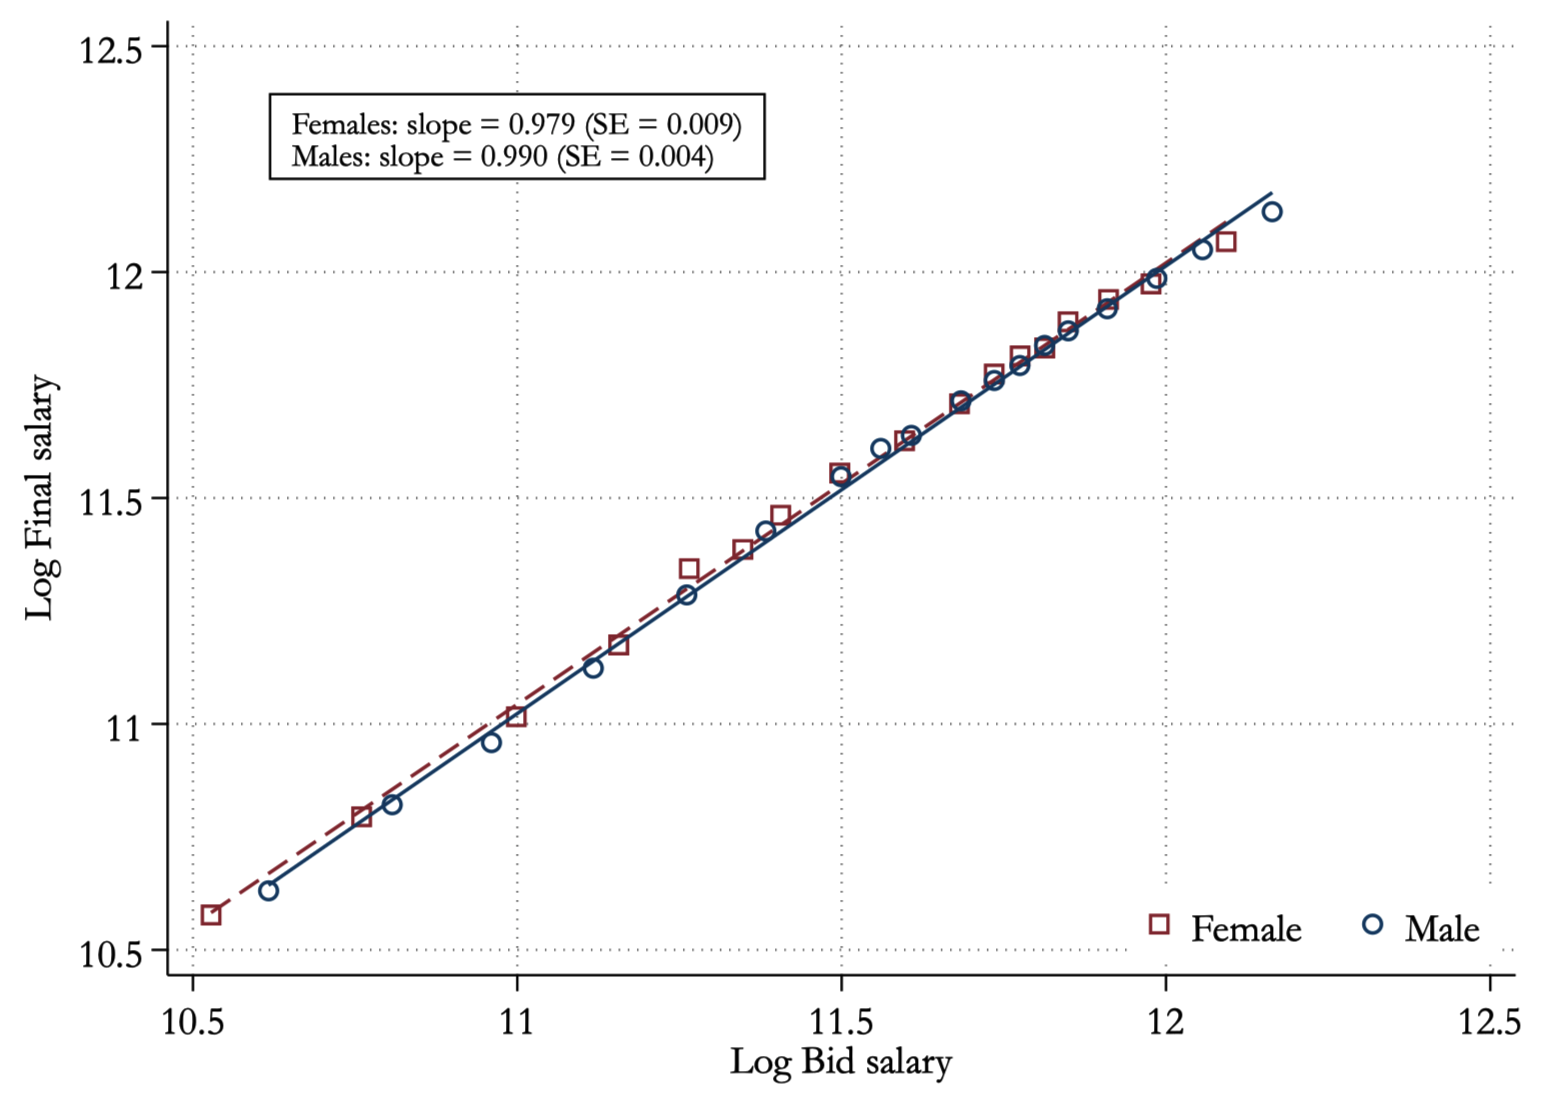
\includegraphics[width = 0.95 \textwidth]{images/bid1.png}
                {\footnotesize \textcolor{frenchlilac!45!white}{Bid} Salary - \textcolor{frenchlilac!45!white}{Final} Salary}
            \end{figure}
        \end{column}
    \end{columns}
\end{frame}